\documentclass[12pt]{scrartcl}
\usepackage[ngerman]{babel}


\usepackage{amsmath, amssymb}

\usepackage{array}  % for the tables

\usepackage{nameref}  % for referencing with name

\usepackage{hyperref}  % for hyperlinks

\usepackage{mathrsfs}

\usepackage{graphicx}  % for the images

\usepackage{xcolor, colortbl}

\usepackage{gensymb} % for \degree

\usepackage{pgfplots}

\usepackage{tabto}

\usepackage{ulem} % \uuline

\usetikzlibrary{arrows}

% \usepgfplotslibrary{external}

% \tikzexternalize

\definecolor{Gray}{gray}{0.85}

\setlength{\parindent}{0cm}

\newcommand{\RomanNumeralCaps}[1]
    {\MakeUppercase{\romannumeral #1}}

% hyperlinks
\hypersetup{
    colorlinks,
    citecolor=black,
    filecolor=black,
    linkcolor=black,
    urlcolor=black
}

\bibliographystyle{IEEetran}




\author{David Jäggli}

\title{Diskrete Mathematik - Übungen SW10}



% ---------- Begin Main Document ----------- %


\begin{document}

\maketitle

\tableofcontents

\newpage
\section{Einführung in die Zahlentheorie II}
\textbf{I.)}\\

\begin{align*}
    3 \odot_9 (2 \oplus_9 5)  &=  3 + (7 \mod 9) \mod 9 = 3\\
    3 \odot_10 2 \oplus_9 8 &= (3 + 2 \mod 10) + 8 \mod 9 = 4\\
    (3 \odot_{12} 9) \odot_{12} (3 \oplus_{12} 9) &= 0 \\
    7 \odot_9 2 \oplus_9 4 \odot_9 6+ &= 5 \oplus_9 6 = 2 \\
    ((3 \oplus_9 6) \odot_9 3) \ominus_9 8 &= 0 \ominus_9 8 = 1\\
    3 \odot_8 6 \ominus_8 2 \ominus_8 3 &= 2 \ominus_8 5 = 5\\
\end{align*}

\newpage
\textbf{II.)}\\
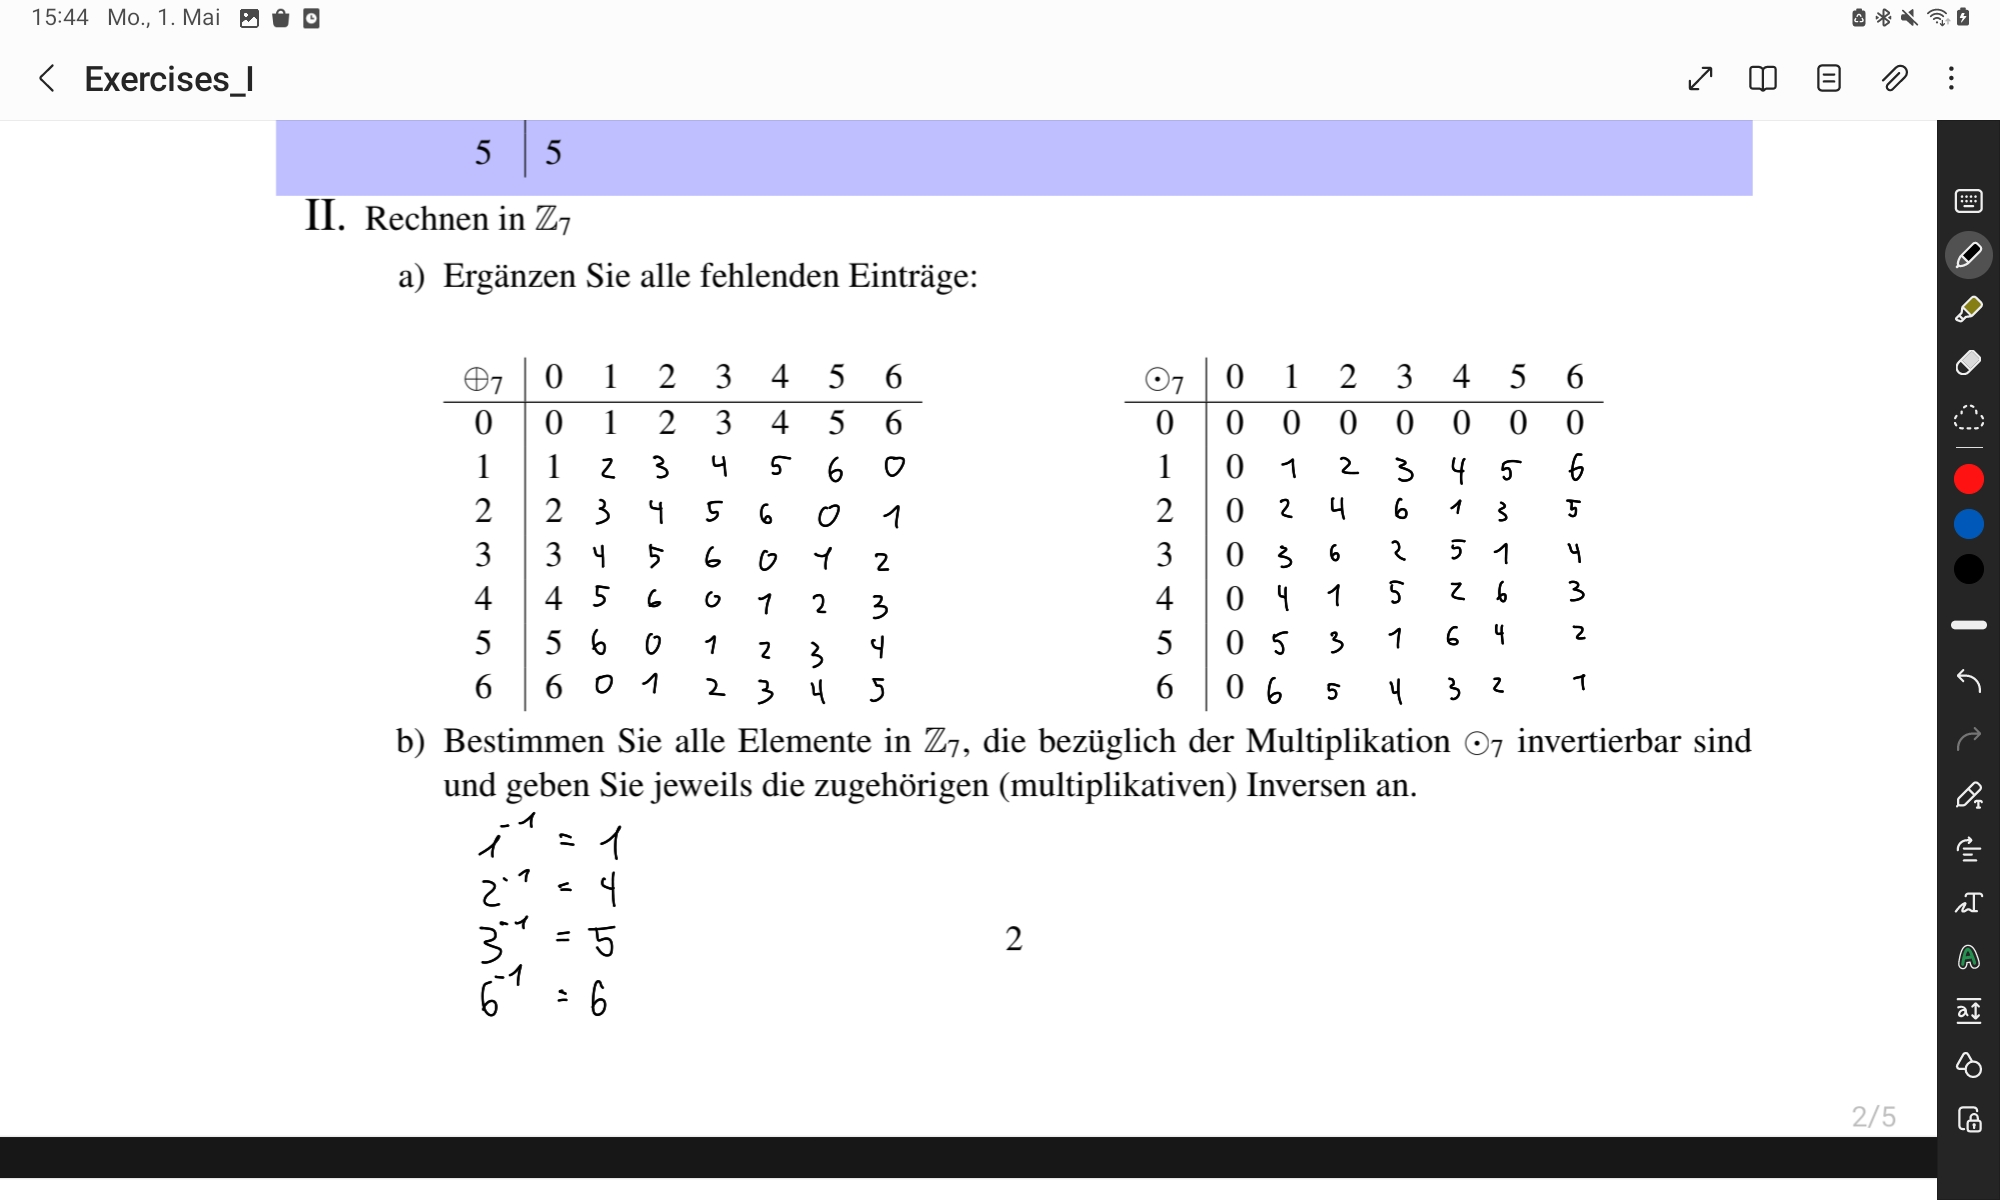
\includegraphics[width=14cm]{img/2_a_b.jpg}

\vspace{1.5cm}
\textbf{III.)}\\
$13 = (1101)_2 \rightarrow QMQMQQQM$\\

$3 \xrightarrow{Q} 9 \xrightarrow{M} 27 \equiv 1 \xrightarrow{Q} 1 \xrightarrow{Q} 1 \xrightarrow{Q} 1 \xrightarrow{M} 3$\\

Da 13 eine Primzahl ist, gilt der kleine Fermat'sche Satz.\\
$3^{13} \mod 13 = 3 \mod 13 = 3$

\vspace{1.5cm}
\textbf{IV.)}\\

\begin{center}
    \begin{tabular}{ c || c | c | c | c | c | c | c | c  }
        $x$                 & 1 & 2 & 4 & 7 & 8 & 11 & 13 & 14\\ 
        \hline
        $x \odot_{15} x$    & 1 & 4 & 1 & 4 & 4 & 1 & 4 & 1\\ 
    \end{tabular}
\end{center}

\begin{center}
    \begin{tabular}{ c || c | c | c | c | c | c | c | c  }
        $a$                 & 1 & 2 & 4 & 7 & 8 & 11 & 13 & 14\\ 
        \hline
        $\sqrt{a} \mod 15$  & 1,4,11,14 & - & 2,7,8,13 & - & - & - & - & -\\ 
    \end{tabular}
\end{center}


\newpage
\textbf{V.)}\\
\begin{center}
    \begin{tabular}{ c || c | c | c | c | c | c | c | c | c | c  }
        $k$             & 1 & 2 & 3 & 4 & 5 & 6 & 7 & 8 & 9 & 10\\ 
        \hline
        $k^2 \mod 11 $  & 1 & 4 & 9 & 5 & 3 & 3 & 5 & 9 & 4 & 1\\ 
    \end{tabular}
\end{center}

QR: 1,3,4,5,9\\
NR: 2,6,7,8,10\\

Nein ist nicht immer so.

\vspace{1.3cm}
\textbf{VI.)}\\
\begin{center}
    \begin{tabular}{ c || c | c | c | c | c | c | c | c | c | c | c | c | c | c | c | c | c | c | c | c}
        $k$             & 1 & 2 & 3 & 4 & 5 & 6 & 7 & 8 & 9 & 10 & 11 & 12 & 13 & 14 & 15 & 16 & 17 & 18 & 19 & 20\\ 
        \hline
        $k^2 \mod 21 $  & 1 & 4 & 9 & 16 & 4 & 15 & 7 & 1 & 18 & 16 & 16 & 18 & 1 & 7 & 15 & 4 & 16 & 9 & 4 & 1\\ 
    \end{tabular}
\end{center}

Alle Reste, welche teilerfremd zu 21 sind:\\
QR: 1,4,16\\
NR: 2,5,8,10,11,13,17,19,20\\

Quadratwurzeln von 1 sind 1,8,13,20\\

\vspace{1.5cm}
\textbf{VII.)}\\
Schlüssel:\\
Alice und Bob haben sich auf $n=13$ und $g=11$ geeinigt. Alice wählt $a=5$ und Bob wählt $b=7$ als 
Geheimzahl\\

a) weis nicht\\

b)
\begin{enumerate}
    \item Alice: $A = g^a \mod n = 11^5 \mod 13 = 7$
    \item Bob: $B = g^b \mod n = 11^7 \mod 13 = 2$
    \item Alice: $k_{BA} = B^a \mod n = 2^5 \mod 13 = 6$
    \item Bob: $k_{AB} = A^b \mod n = 7^7 \mod 13 = 6$
    \item Gemeinsamer Schlüssel: $k = 6$\\
\end{enumerate}

c) Schlüssel ist 6\\



% \begin{align*}
%     1 &= 1 \\
% \end{align*}

% Abschnittsweise definierte Funktionen
% \[ y = g(x) = 
%     \begin{cases} 
%     \frac{1}{2}x    & x \in ]-\infty; -2] \\
%     -2x+3           & x \in ]-2; 3]\\
%     5               & x \in ]3;\infty[
%  \end{cases}
% \]

% Matrix example
% \textbf{Korrektur:}\\
% $\mathbf{A} \odot \mathbf{B} =
% \begin{bmatrix}
%     1 & 1 & 1 \\
%     1 & 1 & 1 \\
%     1 & 0 & 1 \\
% \end{bmatrix}
% $

% tabular example 3 columns
% \renewcommand{\arraystretch}{1.5}
% \begin{center}
%     \begin{tabular}{ | m{12em} | m{12em} | m{12em} | }
%         \hline
%         1 & 2 & 3\\ 
%         \hline
%         1 & 2 & 3\\ 
%         \hline
%         1 & 2 & 3\\ 
%         \hline
%     \end{tabular}
% \end{center}


% tabular example 2 columns
% \renewcommand{\arraystretch}{1.5}
% \begin{center}
%     \begin{tabular}{ | m{17em} | m{17em} | }
%         \hline
%         1 & 2\\ 
%         \hline
%         1 & 2\\ 
%         \hline
%         1 & 2\\ 
%         \hline
%     \end{tabular}
% \end{center}

% \bibliography{}

\end{document}